\documentclass[11 pt]{article}
\usepackage{fullpage,amsthm,amsfonts,amssymb,epsfig,amsmath,times,amsthm}
\usepackage{algorithm,algpseudocode}
\usepackage{setspace}


\usepackage{pgf, tikz}
\usetikzlibrary{arrows, automata}

\newtheorem{theorem}{Theorem}
\newtheorem{claim}[theorem]{Claim}




\title{ CMPS 102 --- Quarter  Spring 2017 --  Homework 4}
\author{VLADOI MARIAN}
\date{\today}

\begin{document}
\maketitle



\begin{center}
{\bf I have read and agree to the collaboration policy.Vladoi Marian}\\
{\bf I want to choose homework heavy option.}\\
{\bf Name of students I worked with: Victor Shahbazian and Mitchell Etzel }
\end{center}


\section*{Solution to Problem 3: Flow decomposition}
Assume that we have a set of paths (P)  connecting source node (s) and sink node (t). Let  $p_i$ be one of the paths $\in$ P. We know that for each $p_i \in P$ , $f'(p_i) \geq 0 $ is a valid path solution iff for every edge $e \in E, \ \sum_{P:p_i:e \in P} f'(p_i) \leq c(e). $ The value of the flow path solution is $\sum_{p_i \in P} f'(p_i)$.\\
We know that we have a valid acyclic  s-t flow, and f is integral.\\
I will give an iterative algorithm that find a valid flow paths solution .\\
1. We start at source node (s).\\
2. Use Depth-First Search from s .\\ 
3. We traverse in each iteration of the algorithm an edge $e = (u,v) \in E$ from the vertex u to v iff f(e) $>$ 0. \\
4. Because the flow is acyclic we know that in a finite number of iteration we have to reach the sink node (t). At this moment we have a s-t path. \\
5. Let edge $e'$ be the min $\{ f(e') | e' \in p_i \}$ (this edge is the edge that is carrying the min amount of flow in path  $p_i$).  \\
6. We add the flow $p_i$ to our set of path flows P, with f'($p_i$ ) = f(e')\\
7. Then update f(e) = f(e) - f(e') for every edge $ e \in p_i$.\\
8. The algorithm terminates when with a 0 flow coming out of s. (at each iteration on edge in the set P has 0 flow).\\

\textbf{a)} Suppose that some directed cycle C has positive flow on every edge. As I mentioned in my algorithm e' is min $\{ f(e') | e' \in p_i \}$.   Then f' is defined by :  f'(e) = f(e) - e' if e $\in C$, or f'(e) = f(e) if e $\notin C$ . We can prove that f' is still a flow and $|f'| = |f|.$\\
If f is acyclic, f(e) = 0 must hold for all $e \in E$ at termination. \\
 Assume for contradiction that some edge e has f(e) $>$ 0. \\
 If we have positive flow out of s, then by flow conservation , we can traverses edges on the path and reach t. Assume that we do not have a possitive flow out of s. If e is an edge $\notin out(s)$, and has f(e) $>$0, we can traverse all the edges in reverse direction and create a cycle, which is a contradiction.\\
Since f is initialy integral, and f'($p_i$) = f(e')  is integral at each iteration, the updated flow f'(e) = f(e) - e' is also integral. Therefore f'$ \{p_i | p_i \in P \}$ are all integral. \\ \\


\textbf{b)}The algorithm terminates in m iterations, because at each iteration at least one edege in P is updated to have flow value = 0, and the flow value on an edge never increases.  \\
Given an acyclic flow f , we find an s-t path $p1 \in P$ along which all flow is positive. Our algorithm decrement the flow on each edge of $p_1$. In the same time this operation will also decrement $|f|$. Then we will repeat the procedure for an s-t path on $p_2 \in P$. At the end , we partion f into a colection of s-t paths (P) of cardinality $|f|$.\\ \\


\textbf{c)} So we proved that an acyclic flow f can be represented as a finite combination of path  flows f'.  But if the flow is not guaranteed to be acyclic, then the algorithm is not guarantee to terminate. It is not guaranteed that f(e) = 0 must hold for all $e \in E$ at termination. We might have some edge e $\notin out(s)$ that have f(e) $> $0. As I previous showed, this implies that our path has cycles. Therefore the flow f is a combination of path flows and cycles. It is not a finite combination of path flows, because we can heve infinite paths s - t. \\
Example:


 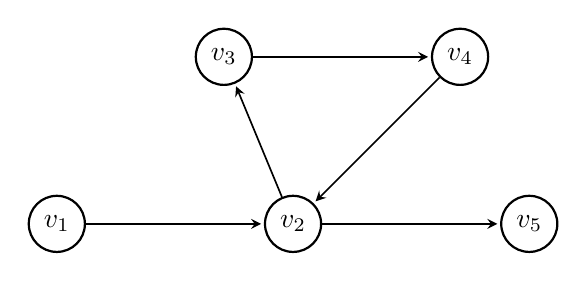
\begin{tikzpicture}[
            > = stealth, % arrow head style
            shorten > = 1pt, % don't touch arrow head to node
            auto,
            node distance = 3cm, % distance between nodes
            semithick % line style
        ]

        \tikzstyle{every state}=[
            draw = black,
            thick,
            fill = white,
            minimum size = 4mm
        ]

        \node[state] (v1) {$v_1$};
        \node[state] (v2) [ right of= v1] {$v_2$};
        \node[state] (v3) [above right of=v1] {$v_3$};
        \node[state] (v4) [right of=v3] {$v_4$};
        \node[state] (v5) [right of=v2] {$v_5$};

        \path[->] (v1) edge node {} (v2);
        \path[->] (v2) edge node{} (v3);
        \path[->] (v3) edge node {} (v4);
        \path[->] (v4) edge node {}(v2);
     \path[->] (v2) edge node{} (v5);

      
    \end{tikzpicture}\\ \\ 
    
    
    Assume that $v_1$ is the source (s)\\
    And $v_5$ is the sink (t).\\
    Then we have an infinite number of paths from $v_1$ to  $v_5$.\\
    $v_1, v_2, v_5$\\
    $v_1, v_2, v_3, v_4, v_2, v_5$.\\
      $v_1, v_2, v_3, v_4, v_2, v_3,v_4,v_2,v_5$.\\
       $v_1, v_2, v_3, v_4, v_2, v_3,v_4,v_2,v_3,v_4,v_2,v_5$.\\
    .....................................................................
\end{document}
